\chapter{基于概率阅读的事件传播模型研究}
\label{chap5:main}
信息传播的\textbf{信息传播模型}分析是社交网络分析中的一个重要研究点,网络热点事件通过社交网络平台迅速传播、发酵,从而在短时间内形成信息爆发、造成极大的影响。社交网络加速了新闻、通知等信息的传播,使得人们接受信息的速率加快,传播信息的成本降低,在一定程度上方便了人们的生活。但是,在社交网络中,人人都可以是信息的生产者、传播者和接收者,每一个社交网络用户都能通过平台发布传播信息。在社交网络中制造舆论热点,进行信息传播的代价相对于传统媒体较低,因此很容易被不法分子利用,对社会安全以及人身财产等造成损失。已有的信息传播模型研究主要包括独立级联模型和线性阈值模型等,这些模型对信息的传播进行了量化,对信息的传播范围进行了传播范围的评估。但是,仍然有一些需求在实际应用中得不到满足。

在信息传播过程中,一个被激活的节点(信息接收者)将尝试继续传播该信息,去激活下一个节点,从而产生级联效应。在实际应用中,一个事件往往由多条主要的信息组成,因此一个事件的传播将由多个传播网络组合而成。所以事件的传播模型首先需要考虑的是多个传播网络的融合问题。其次,社交网络中存在很多的垃圾用户,这些用户活跃度低,或者是由水军控制,会影响到影响力量化的计算,因此需要建立垃圾用户过滤的机制,除去这些干扰噪声。最后,信息的叶子节点,即事件传播的最终的接收者(不再进行下一轮传播)是否阅读到了该信息是概率性的,因此根据用户的社交行为来为用户阅读信息进行建模能够提高影响力量化的准确度。出于精确量化事件传播的影响力的需求,本章提出了一个基于概率阅读的事件传播模型,将多信息传播网络融合、垃圾用户过滤和概率阅读模型综合考虑,为事件在社交网络中的传播进行建模,精确量化事件的传播影响力。

本章的主要工作可以总结如下。首先,基于事件中单条信息的传播网络,我们对多个传播网络进行融合,去除掉重复的节点。其次,利用用户在社交网络中的社交属性,基于逻辑回归模型进行建模,使用梯度下降法进行参数训练,最终得到模型用于垃圾用户过滤。然后,利用用户在社交网络中的时间线上的社交属性,对用户阅读到信息的概率进行建模,对概率阅读模型进行参数训练,得到的模型最终用来预测用户阅读到信息的概率。最后,本章对提出的模型进行了验证,实验使用新浪微博的真实数据集,实验结果证明了模型的有效性。

本章的内容组织如下:第\ref{sec5:motivation}节介绍本章的研究动机,讨论了传统的传播模型的不足之处以及研究基于概率阅读的事件传播模型的意义。第\ref{sec5:definition}节介绍了相关的定义,对本章中所研究的问题进行了定义。第\ref{sec5:method}节介绍了方法描述,详细地阐述了本章提出的模型以及建立过程。第\ref{sec5:experiment}节进行了实验分析,通过实验结果验证了模型的正确性,并对实验结果进行了分析。最后,第\ref{sec5:conclusion}节对本章进行了总结。
\section{研究动机}
\label{sec5:motivation}
在Web 2.0时代,社交网络媒介逐渐开始取代如同报刊、杂志、新闻等传统媒介,占据了信息传播的主导位置。随着各大社交网站的发展,如国外的脸书(Facebook)、推特(Twitter)等,国内的新浪微博、腾讯微博等。与此同时,传统媒介也开始结合社交网络媒介,纷纷开设自己的公共主页,通过互联网及时发布信息,将信息在第一时间推送给用户。在不如大数据时代后,各大社交网络门户的用户呈现几何式爆炸增长的趋势,一条信息通过网络平台在短时间内能够传播影响到的数以百万计的用户。相比于传统媒介,社交网络媒介在信息传播过程中的传播效率与传播范围都大大增强,然而一些虚假信息通过社交网络媒介的传播也能在短时间内迅速扩散,从而可能造成社会的恐慌、用户财产的损失等问题。因此,在大数据时代,社交网络媒介中的信息传播问题成为了信息安全领域的一个研究热点。

信息传播模型定义了社交网络中影响力传播的方式和机制,是研究社交网络中事件传播影响的基础。已有的研究对传播模型做出了深入的研究,其中广泛应用的模型主要有\textbf{独立级联模型}(\textit{Independent Cascade Model})\upcite{goldenberg2001talk,Goldenberg2001Using}和\textbf{线性阈值模型}(\textit{Linear Threshold Model})\upcite{Granovetter1986Threshold,granovetter1983threshold},这两种模型分别从不同的角度描述了信息传播的过程。

独立级联模型是一种概率传播模型,源于市场营销模型研究。独立级联模型基于概率,每一个传播节点在自身转变为活跃状态后,都可以以一定的概率取激活其后继节点,并且多个活跃节点试图影响同一个邻居节点的事件是独立的,所以称之为独立级联模型。独立级联模型是一种比较经典的模型,适用范围广,能够诠释大多数情况的信息传播过程。

线性阈值模型主要源于节点的特异性研究,模型核心出发点为节点的激活阈值,多个活跃节点试图影响同一后继节点的过程是非独立的,节点激活的成功与否取决于多个节点的加权影响是否超过后继节点的阈值。线性阈值模型体现了信息传播过程中影响的累积效应特性,即节点对后继节点的影响是多个节点的累积。

除了上述的信息传播模型外,目前还有一些其他的信息传播模型研究。最为简单的模型是\textbf{统一模型}(\textit{Uniform Model}),模型假设所有节点的传播影响概率都是一个常数,例如0.01。该模型不考虑节点之间的关系,即边的关系。所有的节点对其邻居节点的影响是相同的,不根据结构的变化而变化。此外,模型还假设一个节点对于其所有的邻居节点的影响也是相同的,即不区分邻居节点之间的差别。很显然,这两个假设在实际应用中都是不能得到满足的。基于统一模型的改进为\textbf{三态模型}(\textit{Trivalency Model}),该模型对统一模型中的第一个假设进行了修正。三态模型不再假设所有的节点的传播影响概率是相同的,节点的传播影响概率是均匀随机地从预先设置的概率集合中选取,例如$\{0.001,0.01,0.1\}$。在统一模型中,每一个节点的传播影响概率是相同的,不可区分的。而在三态模型中,节点的传播影响概率是不同的,是可区分的。三态模型的核心思想是将节点的传播影响概率进行了区分,例如传播影响概率为0.001的节点对应于低影响力的节点,传播影响概率为0.01的节点对应于中影响力的节点,传播影响概率为0.1的节点对应于高影响力的节点。在统一模型和三态模型中,节点的传播影响概率都与网络的结构不相关。在\textbf{加权独立级联模型}(\textit{Weighted Independent Cascade})中,传播影响概率与网络的边相关,即与用户关系相关。传播影响概率定义为$p_{u,v}=1 / d_{in}\left(v\right)$,其中$d_{in}\left(v\right)$为节点$v$的入度。该模型相比于上述的两种模型能够更好地诠释信息在社交网络中的传播过程,对于网络中的节点进行了深层次的区分。入度小的节点受到每个入读邻居节点的影响要大于入度大的节点受到的影响,传播影响概率不是简单地从一个常数集合中选取,而是与网络结构相关。另一方面,节点对于其出度邻居节点的传播影响概率不一定是相同的,这是由于出度邻居节点的入度不同。尽管加权独立级联模型拥有以上良好的特性,然而模型的传播影响概率的计算方法仍然缺乏理论保证,传播影响概率与网络的结构相关,但是没有考虑节点之间的历史传播影响概率。\textbf{选举模型}(\textit{Voter Model})\upcite{evendar2011a}是一种广泛应用在统计物理和粒子系统中的一种模型。在选举模型中,各节点随机选取其某一个前驱节点的状态作为自己的状态。上述的各种模型都对信息传播过程的特点进行了研究和建模,为传播分析提供了理论依据,奠定了研究基础。

在社交网络中,独立级联模型最为适应于社交网络的特性。以微博为例,信息的发布源为某个用户,称之为博主。博主发布的博文将推送至博主所有的粉丝,而粉丝接收到此信息后,将以一定的概率转化为激活状态(即转发此条博文)。如果粉丝转发了博文,则其粉丝又会接收到该信息,进而产生级联效应,促使更多的用户接收到该信息。

社交网络具有自身的特性,特别是进入大数据时代后,平台中的信息量庞大。网络中的节点接收到前驱节点信息的概率与该节点所有的前驱节点的状态有关。以微博为例,用户是否能够接收到其关注用户的信息取决于用户在信息推送时是否处于在线状态,即用户接收信息的概率与信息推送时间和用户在线时间的间隔有关。同时在社交网络中,一些节点的活跃度低,为无效节点,不能将其统计入全局的影响传播中。例如,微博中存在很多的垃圾用户,在计算事件的传播影响力时,需要将其滤出才能还原真实的信息传播过程。传统的信息传播分析主要针对单条博文,而在实际应用中,微博中的一个热点事件往往由多条博文组成。因此,对于事件进行传播分析需要针对多个博文进行分析,对应于信息传播过程中多个信息源的热点。同时,用户阅读到信息的概率与信息的发布时间和接收用户的在线时间的间隔相关,需要建立阅读模型来模拟信息传播过程中特性。本章将针对传统的信息传播模型中存在的不足以及在实际应用中的缺陷,结合多源传播网络融合、垃圾用户过滤和概率阅读模型来进行事件的传播分析。
\section{相关定义}
\label{sec5:definition}
在本小节中,我们对所研究的问题进行详细的描述,并对涉及到的概念进行定义和解释。
\subsection{社交网络的基本定义}
\label{subsec5:socialNetwork}
社交网络是由社会个体成员以及社会个体成员之间的联系组成的一种复杂的关系网络。在相关的社交网络研究中,社交网络通常用图$\mathcal{G}=\left(\mathcal{V},\mathcal{E},\mathcal{W}\right)$来表示。其中节点集合$\mathcal{V}=\{v_1,v_2,\cdots,v_n\}$表示社交网络中的社会个体成员,$n$表示整个网络中个体成员的数目。各个社会个体成员之间的关系由图$\mathcal{G}$的边的集合表示,即$\mathcal{E} \subseteq \mathcal{V} \times \mathcal{V}$,其中$\mathcal{V} \times \mathcal{V}$表示节点的笛卡尔集。社会个体成员之间的关系可以是价值观、合作、关联、亲属、好友等各种类型的关系。社会个体的权重以$\mathcal{W}=\{w_1,w_2,\cdots,w_n\}$来表示,用于表示社会个体成员的重要性,例如影响力、公信力等等特征。

\begin{figure}[!ht]
    \centering
    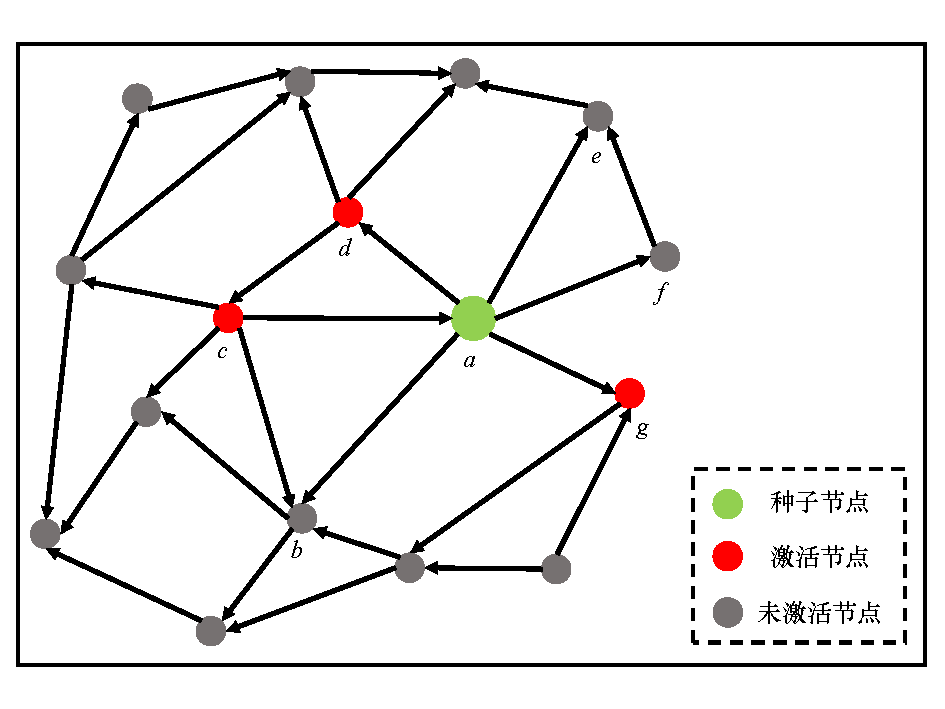
\includegraphics[width=0.8\textwidth]{infoSocial}
    \caption{社交网络中信息传播示意图}
    \label{fig:infoSocial}
\end{figure}

图\ref{fig:infoSocial}给出了社交网络的结构以及信息传播的示意图。信息传播过程可以形式化地描述如下,社交网络中的节点存在两种状态,激活与未激活。在独立级联模型下,给定种子节点后,种子节点首先被激活,然后会以一定概率去激活其他节点,进而形成级联效应。即当节点$u$被激活后,状态由未激活转变成激活,然后节点$u$会以一定的概率去激活处于未激活状态下的邻居节点。如若激活成功,则邻居节点将由未激活状态转变为激活状态,并具备传播能力。如图\ref{fig:infoSocial}中所示,节点$a$为种子节点,在信息传播一开始时被激活,节点$a$在被激活后将以一定的概率去激活其邻居节点$b$、$d$、$e$、$f$、$g$。假设传播情况如图中所示,节点$c$、$d$、$g$被激活,节点$e$、$f$未被激活。由为激活状态转变成激活状态这一过程是不可逆的,这种由未激活状态转变成激活状态的过程称之为信息传播过程。

在社交网络中用户之间的关系主要分为两种,有向关系与无向关系。有向关系表示节点与节点之间的关系是有向的,例如新浪微博、推特中的关注关系。无向关系表示节点与节点之间的关系是无向的,例如脸书中的好友关系。二者的不同之处在于有向图中节点与节点的关系是单向的,可以用有向图表示。而无向关系中节点与节点之间的关系是双向的,可以用无向图表示。特别地,无向关系可以用双向的有向关系来表示。例如,如果节点$u$关注节点$v$,但是节点$v$不一定关注节点$u$。如果节点$u$与节点$v$是好友关系,则节点$v$与节点$u$也是好友。在社交网络中,这两种关系都普遍出现,可以用不同的图结构来表示。

\subsection{独立级联模型}
\label{subsec5:icModel}
Gruhl等人\upcite{gruhl2004information}首先信息传播模型的传播概率的学习进行了研究,Saito等人\upcite{saito2008prediction}研究了独立级联模型下的信息传播概率。独立级联模型中各个节点之间的影响是相互独立的,每个节点成为激活节点后都有一定的概率来激活其邻居节点。多个节点对同一个节点的激活是相互独立的。

在给定一个初始种子节点集合$S$后,在独立级联模型下信息传播的过程如下所示。在时刻$t=0$,社交网络中节点仅有集合$S$中的节点被激活,其余的节点为非激活状态。如果节点$u$在在时刻$t$被激活,则节点$u$由未激活状态转变成激活状态。在$t+1$时刻,节点$u$将有能力激活其后继节点。假设节点$u$存在一个后继节点$v$,令节点$u$激活节点$v$的概率为$p_{u,v}$。如果节点$u$在$t+1$时刻成功激活节点$v$,则节点$v$由未激活状态变成激活状态,在$t+2$时刻,节点$v$将有能力去激活其后继节点。如果节点$v$未被激活,则会保持未激活状态,但是节点$v$可能在未来的时刻由其他的前继节点激活。信息传播过程将持续到没有节点被激活的时刻为止。

假设$\mathcal{G}=\left(\mathcal{V},\mathcal{E}\right)$为一个社交网络。定义\textbf{信息传播时序}(\textit{information diffusion episode})为一个时间序列$\langle D\left(0\right), D\left(1\right), \cdots, D\left(T\right) \rangle$,且满足条件$D\left(i\right) \cap D\left(j\right) = \emptyset$。其中$T$代表着整个信息传播过程的持续时间,$D\left(t\right)$表示在时间$t$时刻被激活的节点集合。$D\left(0\right)$表示在时间$t=0$时刻被激活的节点,即初始的种子节点集合。约束$D\left(i\right) \cap D\left(j\right) = \emptyset$保证了已经激活的节点不会再变成未激活状态。信息传播过程将持续到$T$时刻结束,其中$D\left(T\right) = \emptyset$,即没有新的节点被激活时,信息传播过程结束。

\begin{figure}[!ht]
    \centering
    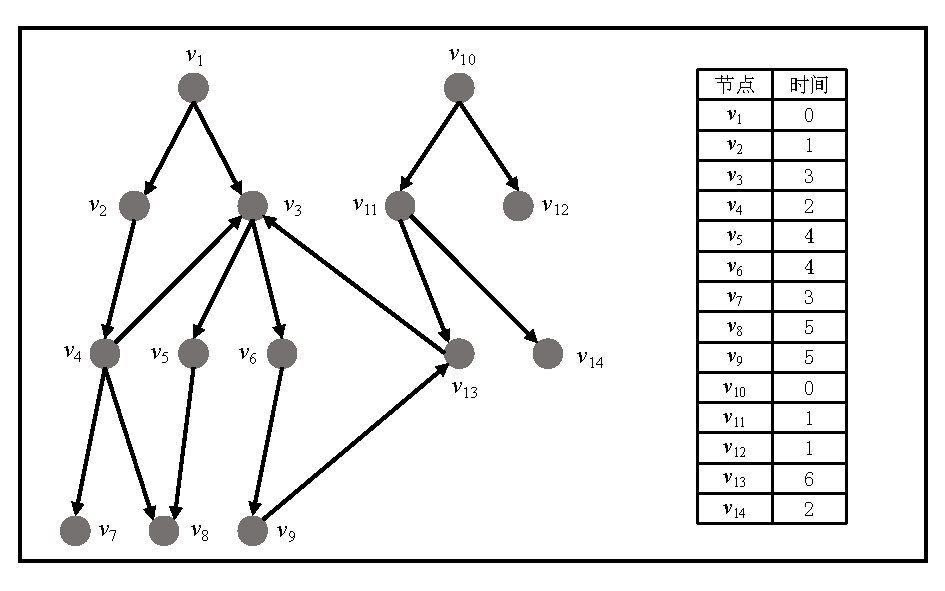
\includegraphics[width=1\textwidth]{infoDiffIC}
    \caption{独立级联模型下信息传播过程示意图}
    \label{fig:infoDiffIC}
\end{figure}

图\ref{fig:infoDiffIC}给出了一个独立级联模型下的信息传播过程的例子。节点$v_1$与节点$v_{10}$为种子节点,故$D\left(0\right)=\{v_1,v_{10}\}$。下一时刻,节点$v_1$激活节点$v_2$,节点$v_{10}$激活节点$v_{11}$和节点$v_{12}$,因此$D\left(1\right)=\{v_2,v_{11},v_{12}\}$。因为$D\left(1\right) \neq \emptyset$,所以信息传播继续进行。按照传播的规则,在$t=2$时刻,$D\left(1\right)$中的节点将有概率激活其后继节点,因此$D\left(2\right)=\{v_4,v_{14}\}$。在$t=3$时刻$D\left(3\right)=\{v_3,v_7\}$,在$t=4$时刻$D\left(4\right)=\{v_5,v_6\}$,在$t=5$时刻,$D\left(5\right)=\{v_8,v_9\}$,在$t=6$时刻,$D\left(6\right)=\{v_{14}\}$。而在$t=7$时刻,$D\left(7\right)=\emptyset$,信息传播过程结束。

\subsection{事件的传播}
\label{subsec5:affair}
基于社交网络的定义以及独立级联模型,我们以新浪微博为例,对社交网络中的事件传播进行研究分析。社交网络中的事件是指在特定的时间区间内,对某一个热点事件进行套路的博文集合。信息通过初始的几个信息源引发更多的人参与讨论和传播,从而影响到更多的社会个体。我们对微博中的事件作形式化的定义,如定义所示。

\begin{mydef}[事件]
\label{def:event}
社交网络中的事件是在一个时段内对同一个主题的信息的集合,与时间和内容相关。令$A$表示事件,则$A=\{a_1, a_2, \cdots, a_n\}$,其中$a_i$为讨论事件$A$的一条信息,由某一个用户发布,而事件$A$中的多条信息可能由同一个人发布。
\end{mydef}

在新浪微博中,事件在用户间主要通过阅读行为、评论行为、转发行为等进行传播,这三种行为对于事件传播的影响力贡献有所区别。
\begin{itemize}
  \item \textbf{阅读行为},指用户阅读到了其时间线上的信息,但是没有做出任何相应的相应行为。时间线上的信息有一定概率被用户所阅读到,这个概率与信息发布时间和用户的活跃时间的间隔相关。因此,阅读行为对于事件传播影响力的贡献是概率性的。
  \item \textbf{评论行为},指用户在阅读到其时间线上的信息后,对信息进行了评论,可以看作是一种特殊的阅读行为,即阅读到该信息的概率为1。因此,评论行为对于事件传播影响力的贡献是确定性的,但是信息的传播在该节点终止,不能产生进一步的传播,即不能产生级联效应。
  \item \textbf{转发行为},指用户阅读到时间线上的信息后,对信息进行了转发,即自身也变成了一个传播源。转发行为不仅对于事件传播影响力的贡献是确定性的,而且转发信息的用户自身也具备了传播能力,产生了级联效应。
\end{itemize}

由上可以看出不同的行为对于事件的传播影响的贡献是不同的,针对不同的用户的行为,需要按照不同的计算方式来衡量其对于事件传播影响力的贡献。在独立级联模型下事件的初始种子节点集合为发布事件中信息的用户集合。令发布事件中信息的用户集合为$S=\{s_1,s_2,\cdots,s_k\}$,其中$s_i$为某个用户,则初始种子节点集合为$S$。在信息传播过程中,转发信息的用户在转发行为的时刻转变为激活节点,具备传播信息的能力,即可能激活其他的用户变为激活状态,形成级联效应。

\begin{figure}[!ht]
    \centering
    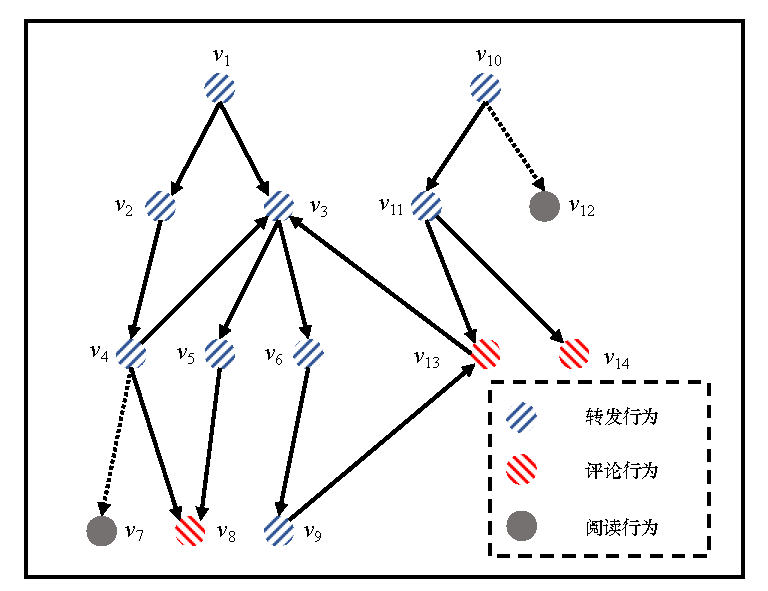
\includegraphics[width=0.9\textwidth]{affairInf}
    \caption{不同行为对于事件传播影响力的贡献}
    \label{fig:affairInf}
\end{figure}

如图\ref{fig:affairInf}所示,图中为三种行为在事件的传播中对影响力的贡献示意图。例如节点$v_4$转发了节点$v_2$发布的信息,则节点$v_4$对于事件传播影响力的贡献是确定性的,并且节点$v_4$具备了传播信息的能力。节点$v_7$以一定的概率阅读了节点$v_4$发布的信息,故$v_7$对于事件的传播影响力贡献是概率性的。节点$v_8$评论了节点$v_4$发布的信息,故$v_8$对于事件的传播影响力贡献是确定性的。故计算事件在图\ref{fig:affairInf}中的传播影响力为计算三种行为对于传播影响力的贡献。令$I\left(A\right)$表示事件$A$的传播影响力,定义其为影响到的节点的数目。假设途中节点$v_7$阅读到信息的概率为0.6,节点$v_12$阅读到信息的概率为0.4,则事件的传播影响力$I\left(A\right)=13$。

在计算事件的传播影响力时,转发行为和评论行为的贡献是确定性的,而阅读行为是概率性的。因此,相对于传统的模型,需要对用户阅读到信息的过程进行建模。
\section{方法描述}
\label{sec5:method}
事件传播影响力的计算与传统模型的传播影响力的计算相比,面临如下几个问题。首先是多条信息的传播网络图的融合。根据定义\ref{def:event},事件由多条信息组成,因此事件的信息源是多源的。其次,社交网络中存在着很多垃圾用户,这些用户对于事件的传播影响力计算会造成干扰,因此需要将垃圾用户进行滤除。然后,阅读行为为一种概率性的行为,概率与信息发布的时间和用户的活跃时间的间隔相关。因此需要对阅读行为进行建模。
\subsection{事件传播网络融合}
\label{subsec5:mix}
在给定了事件$A=\{a_1, a_2, \cdots, a_n\}$后,我们可以根据组成事件的信息的源节点得到种子节点集合$S=\{s_1,s_2,\cdots,s_k\}$。每一个种子节点$s_i$的传播都是一个网络,而微博用户之间的网络拓扑结构是一个高集聚性的复杂网络,种子节点$s_i$的后继节点中会有大量相同的节点。因此,在进行多源信息传播网络融合时需要对重复的网络节点进行去重。

得到种子节点集合后,可以利用新浪微博提供的API爬取种子节点的粉丝,即后继节点。然后,对于转发或者评论事件$A$中不同的信息$a_i$而形成的边进行去重。事件传播网络融合的算法可以描述如算法\ref{alg:affairDiff}所示,

\begin{algorithm}[!ht]
    \caption{$Merge(A,S)$}
    \label{alg:affairDiff}
    \begin{algorithmic}[1]
	\REQUIRE $A,S$
    \ENSURE $\mathcal{G}$
    \STATE initialize $\mathcal{G}=\left(\mathcal{V},\mathcal{E}\right)$, $\mathcal{V}=\emptyset$, $\mathcal{E}=\emptyset$
    \STATE initialize $Q = \emptyset$
    \FOR{$s_i \in S$}
    		\STATE $\mathcal{V} = \mathcal{V} \cup \{s_i\}$
    	\ENDFOR
    	\FOR{$a_i \in A$}
    		\STATE $v = pop\left(a_i\right)$
    		\IF{$v \notin Q$}
    			\IF{$v \in Q_{repost}\left(a_i\right)$ and $e_{u,v} \notin \mathcal{E}$}
    				\WHILE{$Q_{repost}\left(a_i\right) \neq \emptyset$}
    					\STATE $Q = Q \cup \{v\}$
    					\STATE $\mathcal{V} = \mathcal{V} \cup \{v\}$
    					\STATE $e_{u,v}.p = 1$, $\mathcal{E} = \mathcal{E} \cup \{e_{u,v}\}$
    					\STATE $Q_{repost}\left(a_i\right)=Q_{repost}\left(a_i\right) \cup \{v\}$		
    				\ENDWHILE
    			\ENDIF
    			\IF{$v \in Q_{comment}\left(a_i\right)$ and $e_{u,v} \notin \mathcal{E}$}
    				\STATE $Q = Q \cup \{v\}$
    				\STATE $\mathcal{V} = \mathcal{V} \cup \{v\}$
    				\STATE $e_{u,v}.p = 1$, $\mathcal{E} = \mathcal{E} \cup \{e_{u,v}\}$
    			\ENDIF
    			\IF{$v \in Q_{follwer}\left(a_i\right)$ and $e_{u,v} \notin \mathcal{E}$}
    				\STATE $Q = Q \cup \{v\}$
    				\STATE $\mathcal{V} = \mathcal{V} \cup \{v\}$
    				\STATE $\mathcal{E} = \mathcal{E} \cup \{e_{u,v}\}$
    			\ENDIF
    		\ENDIF
    	\ENDFOR
    \end{algorithmic}
\end{algorithm}

首先对事件传播网络图$\mathcal{G}$进行初始化,对节点集合$\mathcal{V}$和边集合$\mathcal{E}$都赋值为空,如算法中第1行所示。设计一个队列$Q$来记录已经存在的节点,初始值为空,见算法中的第2行。第3行至第5行为将所有的种子节点加入事件传播网络图中。然后算法对事件传播中的三种行为,即转发行为、评论行为和阅读行为分别进行不同的处理。针对转发行为,令$Q_{repost}\left(a_i\right)$表示转发了信息$a_i$的用户集合。如果节点$v$对事件$A$进行了转发且不重复,则算法记录其传播影响,将节点$v$加入到队列$Q$中,更新图$\mathcal{G}$。由于转发行为对于事件传播影响力的贡献是确定性的,故边的权重$e_{u,v}.p = 1$。转发行为使得节点$v$也具备传播能力,故将节点$v$加入队列$Q_{repost}\left(a_i\right)$。针对评论行为,令$Q_{comment}\left(a_i\right)$表示评论了信息$a_i$的用户集合。如果节点$v$对事件$A$进行了评论且不重复,则算法记录其传播影响,将节点$v$加入到队列$Q$中,更新图$\mathcal{G}$。由于评论行为对于事件传播影响力的贡献是确定性的,故边的权重$e_{u,v}.p = 1$。评论行为不能使得节点$v$变成激活状态,故节点$v$不能继续传播。针对阅读行为,令$Q_{follwer}\left(a_i\right)$为发布信息$a_i$的用户$u$的粉丝集合,粉丝阅读到信息是一个概率性的事件,因此对边的权重不能进行赋值,需要进一步的处理,算法仅更新了图$\mathcal{G}$。

通过事件传播网络融合,我们将事件$A$中的多源信息传播网络进行融合,对三种不同的行为分别处理,最终得到事件$A$的传播图$\mathcal{G}=\left(\mathcal{V},\mathcal{E}\right)$。

\subsection{垃圾用户过滤}
\label{subsec5:spam}
在得到事件传播网络图$\mathcal{G}=\left(\mathcal{V},\mathcal{E}\right)$后,节点集合$\mathcal{V}$包含了事件$A$传播过程中影响到的所有节点。但是由于社交网络中不可避免地包含了很多垃圾用户,而这些用户是由程序操控或者是长期未登录的用户,这些用户已经不存在传播或者接收信息的能力。如果将这些用户对事件传播影响力的贡献计算在内,则会造成误差。因此,在计算事件传播影响力时,需要将垃圾用户进行过滤。

目前已有的研究对于垃圾用户判别的方法主要包括基于决策树的方法、基于朴素贝叶斯的方法和基于SVM的方法等。上述的方法都是首先获取用户的社交行为属性,例如关注数、粉丝数、发布信息数等等,然后建立用户模型,即构造分类器,最后利用标注的训练数据集进行参数训练,得到训练参数。在得到训练参数后,即得到分类器后,便可以利用分类器对于新的用户是否为垃圾用户做出预测。

为了解决垃圾用户对于事件传播影响力造成的干扰,本章采用了基于\textbf{逻辑回归模型}(\textit{Logistic Regression Model})的方法进行垃圾用户过滤。逻辑回归模型是一种二元分类模型,如果类别超过两种则需要采用多元逻辑回归模型。逻辑回归模型以sigmoid函数为基础,sigmoid函数如公式(\ref{eq:sigmoid})所示,
\begin{equation}
\label{eq:sigmoid}
	h_ {\bm{\theta}} \left(\mathbf{x}\right) = \frac{1}{1 + e^{-{{\bm{\theta}}^T}\mathbf{x}}}
\end{equation}
其中$\mathbf{x}=\left({x_1},{x_2},\cdots,{x_n}\right)$是用户的社交行为属性,$\bm{\theta}=\left({\theta _1},{\theta _2},\cdots,{\theta _n}\right)$为相应的待训练参数。由公式(\ref{eq:sigmoid})可知$h_ {\bm{\theta}} \left(\mathbf{x}\right) \in \left(0,1\right)$。我们可以定义$h_ {\bm{\theta}} \left(\mathbf{x}\right) = 0$表示用户$\mathbf{x}$为垃圾用户,$h_ {\bm{\theta}} \left(\mathbf{x}\right) = 1$表示用户$\mathbf{x}$为正常用户。因此,在训练逻辑回归模型时,它的耗损函数可以表示如公式(\ref{eq:costFunction})所示,
\begin{equation}
\label{eq:costFunction}
	J\left(\bm{\theta}\right) = \frac{1}{m}\sum_{i=1}^m {Cost\left( h_ {\bm{\theta}}\left(\mathbf{x}_i\right), y_i\right)}
\end{equation}
其中$m$为训练集样本的大小,$\mathbf{x}_i$与$y_i$为训练集中的样本点,$Cost\left( h_ {\bm{\theta}}\left(\mathbf{x}_i\right), y_i\right)$如公式(\ref{eq:cost})所示,
\begin{equation}
\label{eq:cost}
	Cost\left( h_ {\bm{\theta}}\left(\mathbf{x}\right), y\right) = \left\{ \begin{array}{rcl} -\log \left(h_ {\bm{\theta}} \left(\mathbf{x}\right)\right) & \mbox{if} & y=1 \\ -\log \left(1 - h_ {\bm{\theta}} \left(\mathbf{x}\right) \right) & \mbox{if} & y=0  \end{array} \right.
\end{equation}
利用公式(\ref{eq:cost})可以得出整个训练集的损失函数值。模型的训练转化为求解参数$\bm{\theta}$使得损失函数最小化的问题,如公式(\ref{eq:minCostFunc})所示,
\begin{equation}
\label{eq:minCostFunc}
	\bm{\theta}^{\ast} = \arg\min{J\left(\bm{\theta}\right)}
\end{equation}
其中$\bm{\theta}^{\ast}$为求解的最优解。求解$\bm{\theta}^{\ast}$可以使用梯度下降法来求解,求解的算法可以表示如算法\ref{alg:gradient}所示。
\begin{algorithm}[!ht]
	\caption{$Gradient(\mathbf{X},Y)$}
	\label{alg:gradient}
	\begin{algorithmic}[1]
	\REQUIRE $\mathbf{X},Y,\varepsilon,\alpha$
	\ENSURE $\bm{\theta}^{\ast}$
	\STATE initialize $\bm{\theta}$
	\STATE{$\bm{\theta}' = \bm{\theta} - \alpha \frac{\partial J\left(\bm{\theta}\right)}{\partial \bm{\theta}}$}
	\WHILE {$\vert J\left(\bm{\theta}'\right) - J\left(\bm{\theta}\right)\vert > \varepsilon$}
		\STATE {$\bm{\theta} = \bm{\theta}'$}
		\STATE {$\bm{\theta}' = \bm{\theta} - \alpha \frac{\partial J\left(\bm{\theta}\right)}{\partial \bm{\theta}}$}
	\ENDWHILE
    \end{algorithmic}
\end{algorithm}

其中$\mathbf{X},Y$表示训练集,$\mathbf{X}={\mathbf{x}_1, \mathbf{x}_2, \cdots, \mathbf{x}_m}$,$Y = {y_1, y_2, \cdots, y_m}$,$\varepsilon$为设置的阈值,$\alpha$为学习率。$\varepsilon$和$\alpha$都为常数。算法利用梯度下降的方法来搜寻最优解,当满足条件$\vert J\left(\bm{\theta}'\right) - J\left(\bm{\theta}\right)\vert \leq \varepsilon$时找到最优解$\bm{\theta}^{\ast}$。但是该方法可能会陷入局部最优解中,因此,我们需要改变初始值以及学习率,进行若干次最优解的搜索,选择$J\left(\bm{\theta}\right)$的值最小的$\bm{\theta}$作为最优解。

训练得到垃圾用户过滤器后,我们基于事件传播网络图$\mathcal{G}=\left(\mathcal{V},\mathcal{E}\right)$,对于节点集合$\mathcal{V}$中的节点$\mathbf{x}$,我们更新节点的权值为$h_ {\bm{\theta}} \left(\mathbf{x}\right)$,即当节点为正常用户时,我们计算节点对事件传播影响力的贡献为1,当节点为垃圾用户时,我们计算节点对事件传播影响力的贡献为0。而对于中间值的用户,我们以系数$h_ {\bm{\theta}} \left(\mathbf{x}\right)$作为节点对事件传播影响力的贡献。

\subsection{概率阅读模型}
\label{subsec5:readModel}
在得到垃圾用户过滤后的事件传播网络图后,即为每个节点以用户为正常用户的概率赋值,我们可以基于用户的三种不同行为来计算事件传播影响力。其中转发行为和评论行为是确定性的,可以直接计算。而阅读行为是一种概率性的行为,需要根据信息发布时间和用户的活跃时间的间隔来计算。在社交网络中,用户可以接收到的信息来源与该用户关注的用户所发布的信息。每时每刻用户都会接收到大量的信息推送,这些信息在系统中默认按照时间线由近及远地推送给用户,即用户在浏览信息时,首先阅读到的信息是前一时刻发布的信息,以此类推到一段时间以前的信息。因此,用户可能会错过部分推送的信息,例如某些与用户登录时刻间隔比较长的信息。用户在使用搜索引擎的过程中,大部分用户只会浏览返回的检索结果的前几页,阅读到之后检索结果的概率会降低。用户在浏览社交网络推送的信息时也有相同的情况,即大多数用户在阅读该时刻系统推送的前几页信息。一条信息出现在用户时间轴的位置与信息发布时间和用户的活跃时间的间隔以及用户自身时间线中信息的推送速率相关。用户所关注的用户越多,所关注的用户越活跃,信息推送的速率越快,即单位时间内推送的信息数目越多。

为了描述用户概率性的阅读到某条信息这一过程,我们采用类似于高斯分布的函数来模拟用户阅读到信息的概率分布,概率阅读分布如公式(\ref{eq:gauss})所示,
\begin{equation}
\label{eq:gauss}
	p\left(t\right) = \left\{ \begin{array}{rcl} \frac{2}{\sqrt{2 \pi} \sigma}\mathsf{e}^{-\frac{\left(t-\mu\right)^2}{2{\sigma}^2}} & \mbox{if} & t \geq 0 \\ 0 & \mbox{if} & t < 0  \end{array} \right.
\end{equation}
其中$t$为信息发布时间和用户的活跃时间的间隔,$p\left(t\right)$为间隔为$t$的阅读概率。信息发布时间先于用户的活跃时间时,$p\left(t\right) > 0$,信息发布时间晚于用户的活跃时间时,$p\left(t\right) = 0$。$\mu$和$\sigma$为待训练的参数,衡量用户的社交网络行为与阅读概率之间的关系。(此处需要补充一张图)

概率阅读模型的训练即$\mu$和$\sigma$的参数训练,可以利用梯度下降法来训练参数,具体的过程如下。首先,我们得到一个标注的训练数据集,数据集包含若干组信息发布时间和用户的活跃时间的间隔$t$与用户是否阅读到了信息的标志$y$,其中阅读信息标注为1,未阅读信息标注为0。则耗损函数如公式(\ref{eq:costReadFunc})所示,
\begin{equation}
\label{eq:costReadFunc}
	L\left(\mu, \sigma \right) = \frac{1}{m}\sum_{i=1}^m {Cost\left( p\left(t_i\right), y_i\right)}
\end{equation}
其中$Cost\left( p\left(t_i\right), y_i\right)$如公式(\ref{eq:costRead})所示,
\begin{equation}
\label{eq:costRead}
	Cost\left( p\left(t_i\right), y_i\right) = \left\{ \begin{array}{rcl} -\log \left(p\left(t\right)\right) & \mbox{if} & y=1 \\ -\log \left(1 - p\left(t\right) \right) & \mbox{if} & y=0  \end{array} \right.
\end{equation}

概率阅读模型的参数训练问题转化为一个参数的优化问题,即计算最优的$\mu$和$\sigma$使得损失函数$L\left(\mu, \sigma \right)$最小化,如公式(\ref{eq:readProblem})所示,
\begin{equation}
\label{eq:readProblem}
    \begin{split}
        &\left(\mu^{\ast},\sigma^{\ast}\right) = \arg\min{L\left(\mu, \sigma \right)}\\
        &s.t.~~\mu > 0, \sigma > 0
    \end{split}
\end{equation}
其中$\left(\mu^{\ast},\sigma^{\ast}\right)$表示最优解,即最终需要计算的参数。该优化问题的求解算法可以表示如算法\ref{alg:gradientRead}所示。
\begin{algorithm}[!ht]
	\caption{$Gradient(T,Y)$}
	\label{alg:gradientRead}
	\begin{algorithmic}[1]
	\REQUIRE $T,Y,\varepsilon,\alpha,\beta$
	\ENSURE $\mu^{\ast},\sigma^{\ast}$
	\STATE initialize $\left(\mu,\sigma\right)$
	\STATE{$\left({\mu}',{\sigma}'\right) = \left(\mu,\sigma\right) - \left( \alpha \frac{\partial L\left(\mu, \sigma \right)}{\partial \mu}, \beta \frac{\partial L\left(\mu, \sigma \right)}{\partial \sigma}\right)$}
	\WHILE {$\vert L\left({\mu}',{\sigma}'\right) - L\left(\mu, \sigma \right)\vert > \varepsilon$}
		\STATE {$\left(\mu,\sigma\right) = \left({\mu}',{\sigma}'\right)$}
		\STATE {$\left({\mu}',{\sigma}'\right) = \left(\mu,\sigma\right) - \left( \alpha \frac{\partial L\left(\mu, \sigma \right)}{\partial \mu}, \beta \frac{\partial L\left(\mu, \sigma \right)}{\partial \sigma}\right)$}
	\ENDWHILE
    \end{algorithmic}
\end{algorithm}

其中$T$与$Y$表示训练数据集,$T={t_1,t_2,\cdots,t_m}$,$Y={y_1,y_2,\cdots,y_m}$,$\varepsilon$为设置的阈值,$\alpha$、$\beta$为学习率。$\varepsilon$、$\alpha$和$\beta$都为常数,根据数据集进行调整。算法利用梯度下降的方法来搜寻最优解,当满足条件$\vert L\left({\mu}',{\sigma}'\right) - L\left(\mu, \sigma \right)\vert \leq \varepsilon$时找到最优解$\left(\mu^{\ast},\sigma^{\ast}\right)$。算法\ref{alg:gradientRead}与算法\ref{alg:gradient}一样都会遇到陷入局部最优解的问题,解决方法也是改变初始值以及学习率来进行若干次最优解的搜索,选择$L\left(\mu, \sigma \right)$较小的$\left(\mu,\sigma\right)$作为最后的最优解。
\section{实验分析}
\label{sec5:experiment}
本章设计了一个基于概率阅读的传播模型研究,利用事件传播网络的融合、垃圾用户过滤以及概率阅读模型来提高对事件传播影响力的评估。这三个步骤为事件传播的计算提供了理论依据,还原了事件传播过程的真实情况,优化了事件传播影响力的计算。实验环境为双核(Intel Xeon 2.40GHz CPU),8GB内存的机器中运行,操作系统为Ubuntu 14.04 64位系统,算法采用Java以及Matlab实现,在JDK 1.8.0\_40环境下编译。本节的实验数据的抓取基于新浪微博开放平台提供的weibo4j SDK进行数据抓取。首先,本节介绍实验的设计,然后对实验结果进行展示与分析。

\subsection{实验设计}
\label{subsec5:settings}
本节中的实验利用新浪微博中抓取的热点事件所包含的相关博文信息作为事件$A$,同时抓取发表这些博文信息的用户的信息,以及转发关系作为信息传播网络,然后通过融合构建事件传播网络图$\mathcal{G}=\left(\mathcal{V},\mathcal{E}\right)$。基于逻辑回归模型的垃圾用户过滤算法,利用爬取标注的51,275个用户作为训练集进行模型训练,得到垃圾用户过滤模型,采取交叉验证对模型进行准确率,召回率等性能的验证。最后对引入概率阅读模型后的传播影响力和传统的独立级联模型的传播影响力进行对比分析,验证了模型的性能。

\subsection{实验结果与分析}
\label{subsec5:resultAnalysis}
对于事件传播网络融合部分,我们比较用户去重的效果,我们将去重后的事件传播网络图$\mathcal{G}=\left(\mathcal{V},\mathcal{E}\right)$与传统的多个单源的信息传播网络图进行对比,比较节点数以及边数等指标。热点事件中由于社交网络的高度集聚性以及用户参与多个信息的传播而干扰传播影响力的计算,该实验用于验证事件传播网络融合能否消除其干扰。

进行事件传播网络融合后,事件传播网络图$\mathcal{G}=\left(\mathcal{V},\mathcal{E}\right)$的结构属性与组成该事件的各条信息的传播图的属性对比如图\ref{fig:duplication}所示。

\begin{figure}[!ht]
    \centering
    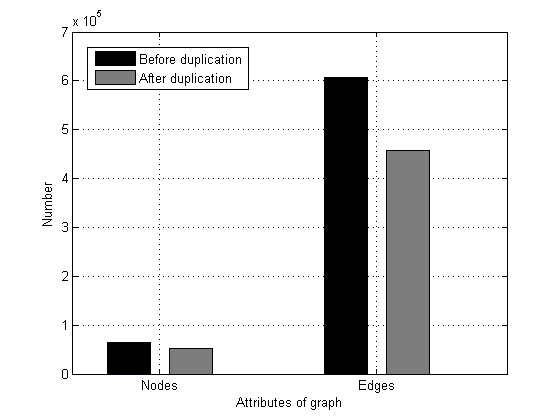
\includegraphics[width=0.7\textwidth]{duplication}
    \caption{事件传播网络融合前后的网络结构属性对比}
    \label{fig:duplication}
\end{figure}

其中横坐标为网络的结构属性,纵坐标为数目。结果图中的深色部分为融合之前多条信息的传播图的属性之和,浅色部分为融合之后的事件传播网络图的属性。从图中我们可以看出,进行融合后,事件传播网络图的节点数和边数都有所下降,其中节点数下降了19.72\%,边数下降了24.76\%。这说明事件传播网络融合在一定程度上能够减少由于重复计算事件中的用户节点数和传播次数而造成的传播影响力计算的误差,由此也可以看出一个热点事件中,存在用户参与到多条信息的传播过程中,而且各条信息形成的传播网络之间存在的交叠,这也从侧面反映了社交网络高度集聚性的特点。

在垃圾用户过滤部分,我们对基于逻辑回归模型生成的垃圾用户过滤器进行验证,利用人工标注好的数据集采用交叉验证的手段进行验证。度量标准采用准确率(\textit{precision})、召回率(\textit{recall})、$F$值以及AUC值\upcite{davis2006the}等指标。

\begin{table}[!ht]
\centering
\caption{垃圾用户过滤中的相关定义}
\label{tab:spam}
\begin{tabular}{ |c|c|c| }
\hline
 & \textbf{垃圾用户} & \textbf{正常用户}\\
\hline
\textbf{真} & $A$ & $B$ \\
\hline
\textbf{假} & $C$ & $D$ \\
\hline
\end{tabular}
\end{table}
在垃圾用户判别的过程中的相关定义如表\ref{tab:spam}所示,其中$A$表示用户为垃圾用户且被正确识别出来的数目,$B$表示用户为正常用户且被正确识别出来的数目,$C$表示用户为垃圾用户但未被正确识别出来的数目,$D$表示用户为正常用户但未正确识别出来的数目。基于上述的定义,准确率、召回率以及$F$值的计算如下所示,
\begin{equation}
\label{eq:spamP}
	P = \frac{A}{\left(A+B\right)}
\end{equation}
\begin{equation}
\label{eq:spamR}
	R = \frac{A}{\left(A+C\right)}
\end{equation}

\begin{equation}
\label{eq:spamF}
	F_\alpha =  \frac{\left(\alpha^2+1\right)PR}{\alpha^2\left(P+R\right)}
\end{equation}
其中$P$为准确率、$R$为召回率以及$F_\alpha$为参数为$\alpha$的$F$值(本节中$\alpha$设置为1)。垃圾用户过滤部分的各指标的结果如表\ref{tab:spamRes}所示。

\begin{table}[!ht]
\centering
\caption{垃圾用户过滤各指标的实验结果}
\label{tab:spamRes}
\begin{tabular}{ |c|c|c|c|c|c| }
\hline
 & \textbf{数据集1} & \textbf{数据集2} & \textbf{数据集3} & \textbf{数据集4} & \textbf{数据集5}\\
\hline
$P$ & 0.9243 & 0.9196 & 0.9292 & 0.9217 & 0.9432 \\
\hline
$R$ & 0.9145 & 0.8882 & 0.9131 & 0.9470 & 0.9502 \\
\hline
$F_1$ & 0.9194 & 0.9036 & 0.9211 & 0.9342 & 0.9467 \\
\hline
$AUC$-$PR$ & 0.9113 & 0.8869 & 0.9103 & 0.9427 & 0.9551 \\
\hline
$AUC$-$ROC$ & 0.8943 & 0.8807 & 0.8918 & 0.9175 & 0.9307 \\
\hline
\end{tabular}
\end{table}

我们将数据集分成5份,然后进行交叉验证,即使用4份作为训练集,其余1份当做实验数据集。其中$P$表示准确率,$R$表示召回率,$F_1$表示$\alpha = 1$时的$F$值,$AUC$-$PR$表示$PR$曲线下的面积,$AUC$-$ROC$表示$ROC$曲线下的面积。有结果可知,垃圾用户的判别准确率和召回率都达到了不错的效果即算法将一个正常用户误判成垃圾用户和将一个垃圾用户误判成正常用户的几率都比较小。而且$F$值的结果显示了算法\ref{alg:gradient}在判断垃圾用户时,准确率和召回率没有存在某一个指标特别差的情况,这说明算法的均衡性较好。

算法的$AUC$-$PR$曲线和$AUC$-$ROC$曲线如图\ref{fig:auc_pr}及图\ref{fig:auc_roc}所示。

\begin{figure}[!ht]
   \begin{minipage}{0.48\textwidth}
     \centering
     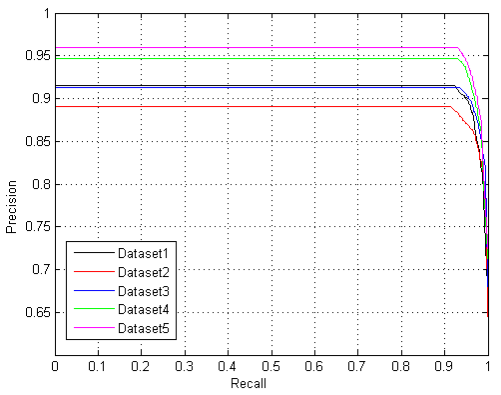
\includegraphics[width=\linewidth]{auc_pr}
     \caption{各数据集的$AUC$-$PR$曲线图}
     \label{fig:auc_pr}
   \end{minipage}
   \hfill
   \begin {minipage}{0.48\textwidth}
     \centering
     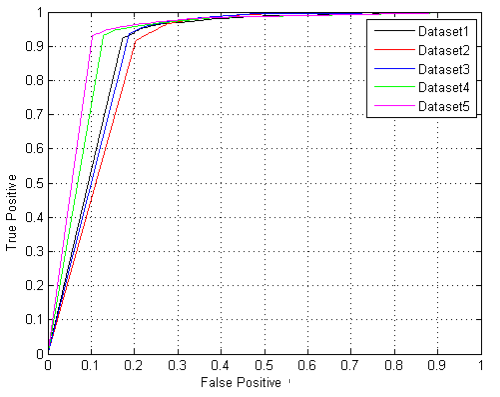
\includegraphics[width=\linewidth]{auc_roc}
     \caption{各数据集的$AUC$-$ROC$曲线图}
     \label{fig:auc_roc}
   \end{minipage}
\end{figure}

图\ref{fig:auc_pr}中横坐标为召回率,纵坐标为准确率。从图中可以看出当召回率超过一定数值时准确率才开始下降,即曲线下的面积较大,说明模型在准确率和召回率两方面的表现都满足了要求。图\ref{fig:auc_roc}的横坐标为假正类率,即分类器错认为正类的负实例占所有负实例的比例,纵坐标为真正类率,即分类器所识别出的正实例占所有正实例的比例。从图中可以看出当假正类率较小的时候,真正类率已经上升到较高的比例,即曲线下的面积较大,说明模型的效果是显著的。

从以上的实验结果分析可知,利用用户的社交行为属性基于逻辑回归模型进行进行垃圾用户过滤是有效的。因此,垃圾用户过滤能够有效减少在事件传播中垃圾用户对于事件传播影响力的计算的干扰,能够还原事件真实影响到的用户数,提高传播影响力的计算的准确性。

针对概率阅读模型部分,实验将概率阅读模型与传统的独立级联模型的传播影响进行对比,验证了概率阅读模型是否能够消除用户未阅读到信息给事件传播影响力计算带来的干扰,从而提高传播影响力计算的准确性。实验计算事件传播在概率阅读模型下和独立级联模型下影响到的用户数作对比,实验结果如图所示。

\begin{figure}[!ht]
    \centering
    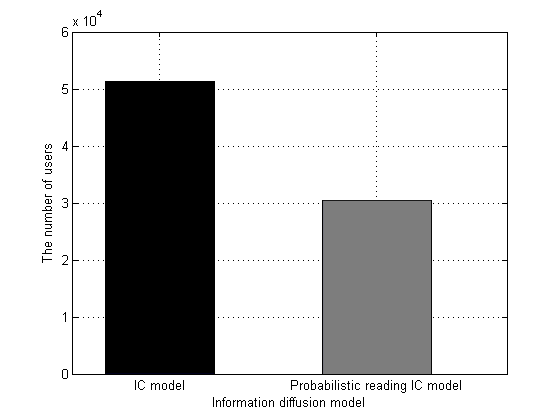
\includegraphics[width=0.7\textwidth]{reading}
    \caption{概率阅读模型与独立级联模型影响用户数目的对比}
    \label{fig:reading}
\end{figure}

由图\ref{fig:reading}可知,事件传播在概率阅读模型下影响到的用户数小于独立级联模型下的用户数。在社交网络中,用户有多种行为来对推送的信息做出反应,转发行为、评论行为以及阅读模型。实验结果说明模型能够反映出用户以一定的概率阅读到关注的用户发布的信息,从而参与到事件的传播中的事实。

社交网络中事件传播影响力的计算问题与传统的信息传播影响力计算有所不同,本节的实验结果证明了所提出的事件传播网络融合、垃圾用户过滤以及概率阅读模型在一定程度上都能提高事件传播影响力的计算。基于概率阅读的事件传播模型能够还原事件传播的过程,对事件传播的过程进行了描述,提高了传播影响力的准确性,还原了事件传播的真实影响力。

\section{本章小结}
\label{sec5:conclusion}
为了更准确地描述社交网络中热点事件的传播过程,本章提出了基于概率阅读的事件传播模型,模型将事件传播网络融合、垃圾用户过滤以及概率阅读模型考虑在内,对于社交网络中事件传播影响力的计算进行了综合考虑。事件传播网络融合对于多源信息传播问题进行了节点去重,减少由于重复计算事件中的用户节点数和传播次数而造成的传播影响力计算的误差。基于逻辑回归模型进行进行垃圾用户过滤能够有效减少在事件传播中垃圾用户对于事件传播影响力的计算的干扰,移除传播过程中的无效用户。概率阅读模型能够反映出用户以一定的概率阅读到关注的用户发布的信息的过程,从而更准确的计算事件的传播影响力。通过新浪微博的数据,我们对所提出的模型的每一个步骤进行了实验,实验验证了所提出模型的有效性。本章所研究的内容对于事件在社交网络中的传播影响力的计算提供了一定的帮助。